% Options for packages loaded elsewhere
\PassOptionsToPackage{unicode}{hyperref}
\PassOptionsToPackage{hyphens}{url}
\PassOptionsToPackage{dvipsnames,svgnames,x11names}{xcolor}
%
\documentclass[
  12pt]{article}

\usepackage{amsmath,amssymb}
\usepackage{iftex}
\ifPDFTeX
  \usepackage[T1]{fontenc}
  \usepackage[utf8]{inputenc}
  \usepackage{textcomp} % provide euro and other symbols
\else % if luatex or xetex
  \usepackage{unicode-math}
  \defaultfontfeatures{Scale=MatchLowercase}
  \defaultfontfeatures[\rmfamily]{Ligatures=TeX,Scale=1}
\fi
\usepackage{lmodern}
\ifPDFTeX\else  
    % xetex/luatex font selection
\fi
% Use upquote if available, for straight quotes in verbatim environments
\IfFileExists{upquote.sty}{\usepackage{upquote}}{}
\IfFileExists{microtype.sty}{% use microtype if available
  \usepackage[]{microtype}
  \UseMicrotypeSet[protrusion]{basicmath} % disable protrusion for tt fonts
}{}
\makeatletter
\@ifundefined{KOMAClassName}{% if non-KOMA class
  \IfFileExists{parskip.sty}{%
    \usepackage{parskip}
  }{% else
    \setlength{\parindent}{0pt}
    \setlength{\parskip}{6pt plus 2pt minus 1pt}}
}{% if KOMA class
  \KOMAoptions{parskip=half}}
\makeatother
\usepackage{xcolor}
\setlength{\emergencystretch}{3em} % prevent overfull lines
\setcounter{secnumdepth}{5}
% Make \paragraph and \subparagraph free-standing
\makeatletter
\ifx\paragraph\undefined\else
  \let\oldparagraph\paragraph
  \renewcommand{\paragraph}{
    \@ifstar
      \xxxParagraphStar
      \xxxParagraphNoStar
  }
  \newcommand{\xxxParagraphStar}[1]{\oldparagraph*{#1}\mbox{}}
  \newcommand{\xxxParagraphNoStar}[1]{\oldparagraph{#1}\mbox{}}
\fi
\ifx\subparagraph\undefined\else
  \let\oldsubparagraph\subparagraph
  \renewcommand{\subparagraph}{
    \@ifstar
      \xxxSubParagraphStar
      \xxxSubParagraphNoStar
  }
  \newcommand{\xxxSubParagraphStar}[1]{\oldsubparagraph*{#1}\mbox{}}
  \newcommand{\xxxSubParagraphNoStar}[1]{\oldsubparagraph{#1}\mbox{}}
\fi
\makeatother


\providecommand{\tightlist}{%
  \setlength{\itemsep}{0pt}\setlength{\parskip}{0pt}}\usepackage{longtable,booktabs,array}
\usepackage{calc} % for calculating minipage widths
% Correct order of tables after \paragraph or \subparagraph
\usepackage{etoolbox}
\makeatletter
\patchcmd\longtable{\par}{\if@noskipsec\mbox{}\fi\par}{}{}
\makeatother
% Allow footnotes in longtable head/foot
\IfFileExists{footnotehyper.sty}{\usepackage{footnotehyper}}{\usepackage{footnote}}
\makesavenoteenv{longtable}
\usepackage{graphicx}
\makeatletter
\def\maxwidth{\ifdim\Gin@nat@width>\linewidth\linewidth\else\Gin@nat@width\fi}
\def\maxheight{\ifdim\Gin@nat@height>\textheight\textheight\else\Gin@nat@height\fi}
\makeatother
% Scale images if necessary, so that they will not overflow the page
% margins by default, and it is still possible to overwrite the defaults
% using explicit options in \includegraphics[width, height, ...]{}
\setkeys{Gin}{width=\maxwidth,height=\maxheight,keepaspectratio}
% Set default figure placement to htbp
\makeatletter
\def\fps@figure{htbp}
\makeatother

\addtolength{\oddsidemargin}{-.5in}%
\addtolength{\evensidemargin}{-1in}%
\addtolength{\textwidth}{1in}%
\addtolength{\textheight}{1.7in}%
\addtolength{\topmargin}{-1in}%
\makeatletter
\@ifpackageloaded{caption}{}{\usepackage{caption}}
\AtBeginDocument{%
\ifdefined\contentsname
  \renewcommand*\contentsname{Table of contents}
\else
  \newcommand\contentsname{Table of contents}
\fi
\ifdefined\listfigurename
  \renewcommand*\listfigurename{List of Figures}
\else
  \newcommand\listfigurename{List of Figures}
\fi
\ifdefined\listtablename
  \renewcommand*\listtablename{List of Tables}
\else
  \newcommand\listtablename{List of Tables}
\fi
\ifdefined\figurename
  \renewcommand*\figurename{Figure}
\else
  \newcommand\figurename{Figure}
\fi
\ifdefined\tablename
  \renewcommand*\tablename{Table}
\else
  \newcommand\tablename{Table}
\fi
}
\@ifpackageloaded{float}{}{\usepackage{float}}
\floatstyle{ruled}
\@ifundefined{c@chapter}{\newfloat{codelisting}{h}{lop}}{\newfloat{codelisting}{h}{lop}[chapter]}
\floatname{codelisting}{Listing}
\newcommand*\listoflistings{\listof{codelisting}{List of Listings}}
\makeatother
\makeatletter
\makeatother
\makeatletter
\@ifpackageloaded{caption}{}{\usepackage{caption}}
\@ifpackageloaded{subcaption}{}{\usepackage{subcaption}}
\makeatother
\ifLuaTeX
  \usepackage{selnolig}  % disable illegal ligatures
\fi
\usepackage[]{natbib}
\bibliographystyle{agsm}
\usepackage{bookmark}

\IfFileExists{xurl.sty}{\usepackage{xurl}}{} % add URL line breaks if available
\urlstyle{same} % disable monospaced font for URLs
\hypersetup{
  pdftitle={Kellogg Finance: Coding Task},
  pdfauthor={William Co},
  colorlinks=true,
  linkcolor={blue},
  filecolor={Maroon},
  citecolor={Blue},
  urlcolor={Blue},
  pdfcreator={LaTeX via pandoc}}


\begin{document}


\def\spacingset#1{\renewcommand{\baselinestretch}%
{#1}\small\normalsize} \spacingset{1}


%%%%%%%%%%%%%%%%%%%%%%%%%%%%%%%%%%%%%%%%%%%%%%%%%%%%%%%%%%%%%%%%%%%%%%%%%%%%%%

\date{January 20, 2025}
\title{\bf Kellogg Finance: Coding Task}
\author{
William Co\thanks{Thank you for the opportunity to complete this data
task for my predoctoral application. I appreciate your consideration,
and I look forward to meeting and contributing.}\\
Department of Economics, University of British Columbia\\
}
\maketitle

\bigskip
\bigskip
\begin{abstract}
This is a data task submitted for a predoctoral application.
\end{abstract}


\newpage
\spacingset{1.9} % DON'T change the spacing!

\section{Introduction}\label{introduction}

A copy of writing sample can be found here
\href{https://github.com/WilliamClintC/EvaluativeAssignment_2024/blob/main/EvaluativeAssignment_2024/Writing\%20Sample.pdf}{link}
and will be submitted as well.
\citep{coEvaluativeAssignment_2024EvaluativeAssignment_2024Writing}

A copy of the time sheet will be submitted

Code and output data for task 2 will be submitted as well.

\section{Task 1: Red Sox Ticket
Prices}\label{task-1-red-sox-ticket-prices}

\emph{How do the prices consumers pay for tickets change as the game
date approaches (i.e., as the number of days between transaction date
and game date declines)? How does this dynamic pattern change across
years?}

To address the question, we begin by running a preliminary regression to
gain a better understanding of our data. This regression includes all
available control variables and accounts for the number of tickets
purchased. Considering the potential for bulk discounts associated with
purchasing multiple tickets, we aim to capture variations in pricing
that may occur in different contexts, where such discounts might or
might not be offered.

\begin{enumerate}
\def\labelenumi{\arabic{enumi}.}
\item
  \textbf{Model with \texttt{number\_of\_tickets}}: \[
  \text{price\_per\_ticket} = \beta_0 + \beta_1 \cdot \text{days\_until\_game} + \beta_2 \cdot \mathbf{\text{controls}}  
  + \beta_3 \cdot \text{num\_tickets} + \epsilon
  \]
\item
  \textbf{Model without \texttt{number\_of\_tickets}}: \[
  \text{price\_per\_ticket} = \beta_0 + \beta_1 \cdot \text{days\_until\_game} + \beta_2 \cdot \mathbf{\text{controls}} + \epsilon
  \]
\item
  \textbf{Model with \texttt{number\_of\_tickets} using log price}: \[
  \log(\text{price\_per\_ticket}) = \beta_0 + \beta_1 \cdot \text{days\_until\_game} + \beta_2 \cdot \mathbf{\text{controls}} + 
  \beta_3 \cdot \text{num\_tickets} + \epsilon
  \]
\item
  \textbf{Model without \texttt{number\_of\_tickets} using log price}:
  \[
  \log(\text{price\_per\_ticket}) = \beta_0 + \beta_1 \cdot \text{days\_until\_game} + \beta_2 \cdot \mathbf{\text{controls}} + \epsilon
  \]
\end{enumerate}

Where: \[
\mathbf{\text{controls}} = \text{day\_game, weekend\_game, sectiontype, gamemonth, team, year}
\]

\begin{itemize}
\tightlist
\item
  \(\beta_0\) is the intercept.
\item
  \(\beta_1, \beta_3\) are the coefficients for the respective predictor
  variables.
\item
  \(\beta_2\) is a vector of coefficients for control variables.
\item
  \(\epsilon\) is the error term.
\end{itemize}

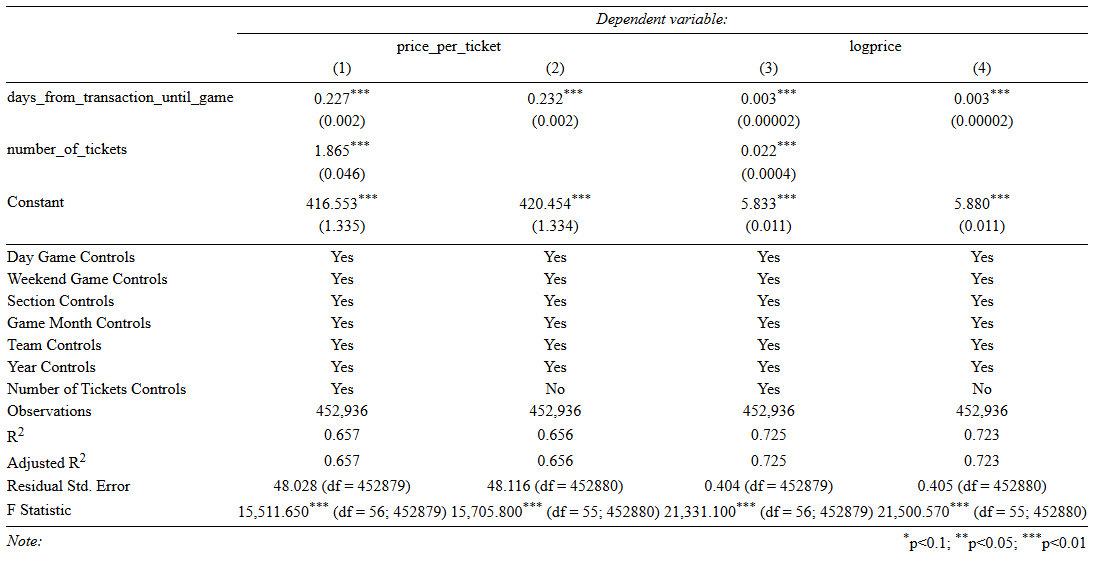
\includegraphics{images/0.png}

The results indicate that the earlier tickets are purchased, the more
expensive they tend to be, as evidenced by the positive and significant
coefficient on the variable
\texttt{days\_from\_transaction\_until\_game}. This finding is counter
intuitive. Typically, purchasing tickets earlier is expected to be less
expensive because it reduces the risk for the ticket vendor, smooths out
their cash flow, and provides an early cash injection. Additionally, the
time value of money suggests that receiving payments earlier should
incentivise lower prices.

To explore this unexpected result further, we conduct an investigation
using scatter plots.

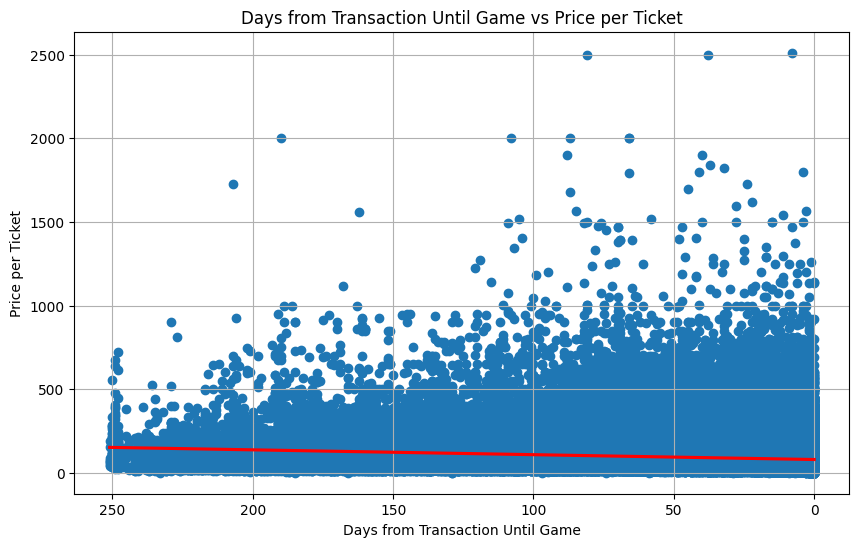
\includegraphics{images/16.png}

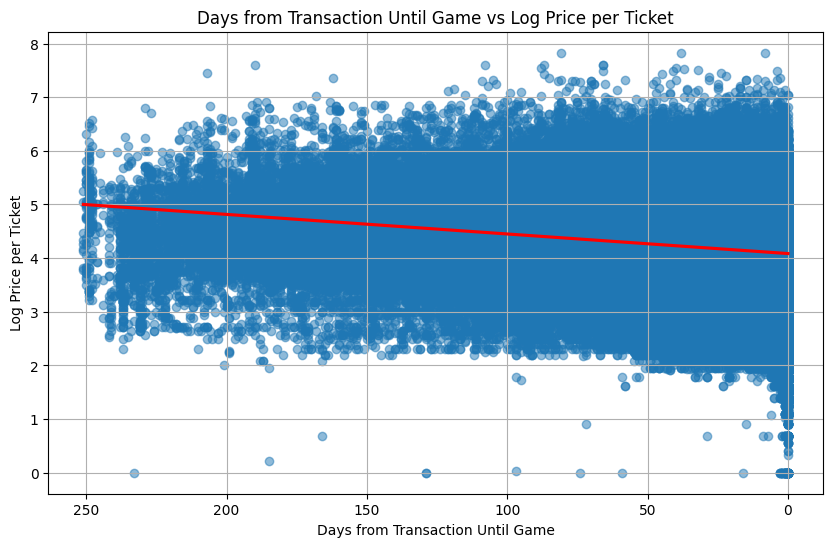
\includegraphics{images/17.png}

The relationship may be biased by noise. So this would warrant further
investigation. To investigate further, I look into the team with the
most observations (NYY). I also control for other attributes with the
most observation within NYY (LowerBleachers, 2 Tickets, April, Evening
and Weekend games in 2011). The following are my
results.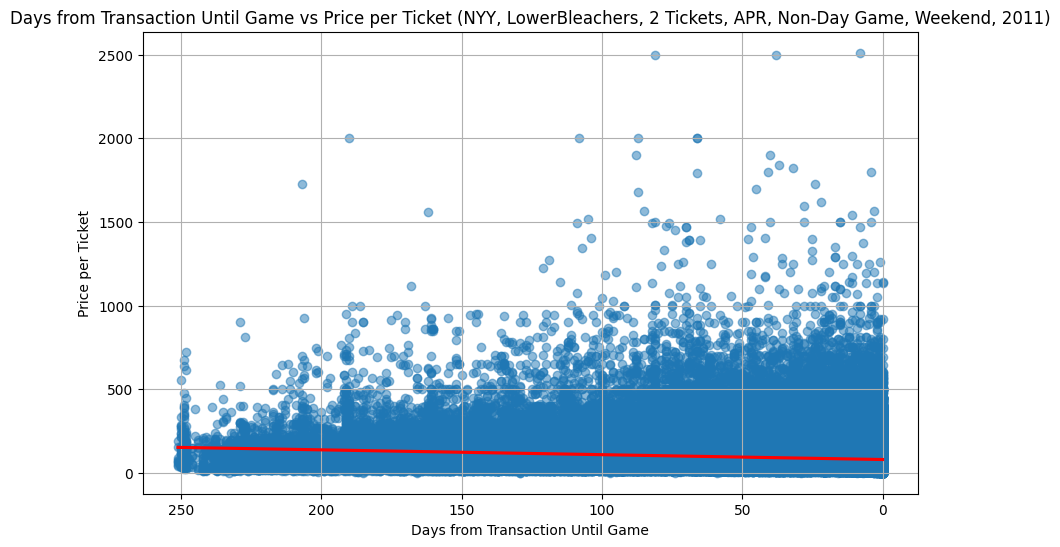
\includegraphics{images/18.png}

The results show similarity to the initial plots we observed from
earlier. I suspect the results from the data are due to some noise
introduced by price outliers. I clean the data of price outliers
manually and rerun the same regressions, mentioned prior.

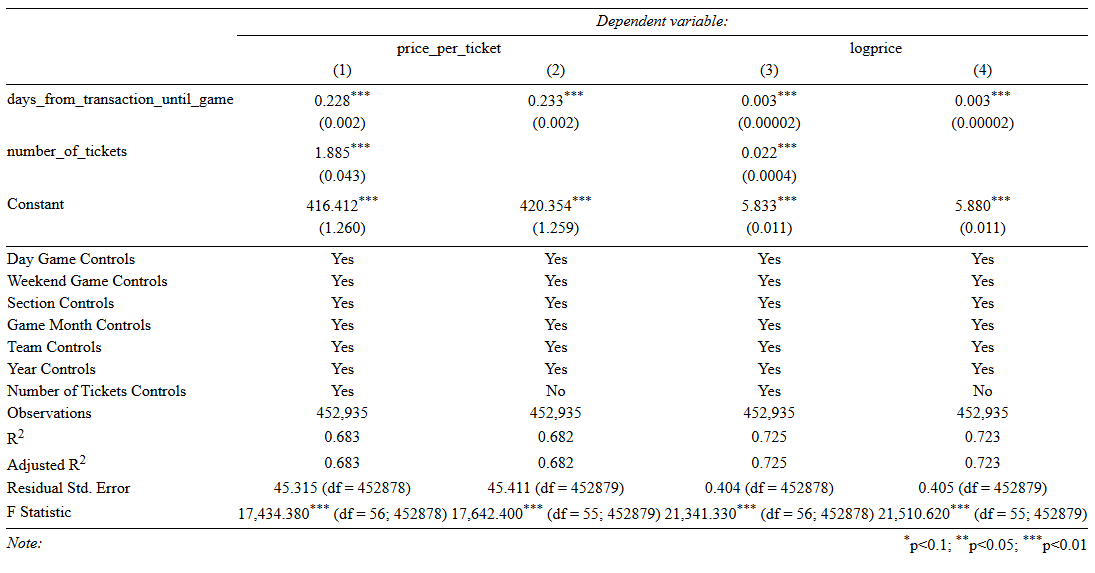
\includegraphics{images/5.png}

There does not seem to be any significant effect on the results. To
further investigate, we use bin scatter plots and show our results
again.

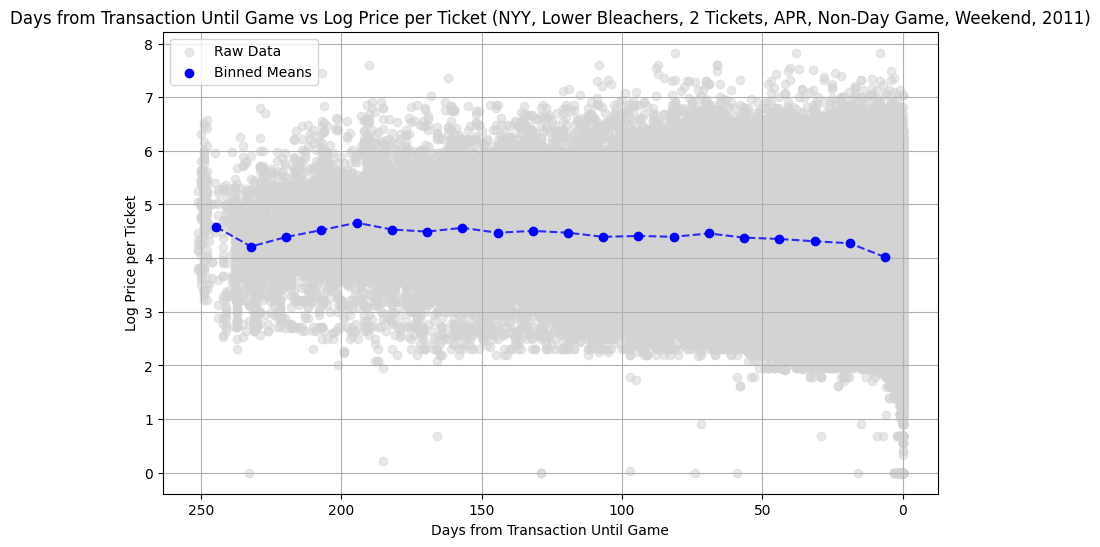
\includegraphics{images/11.png}

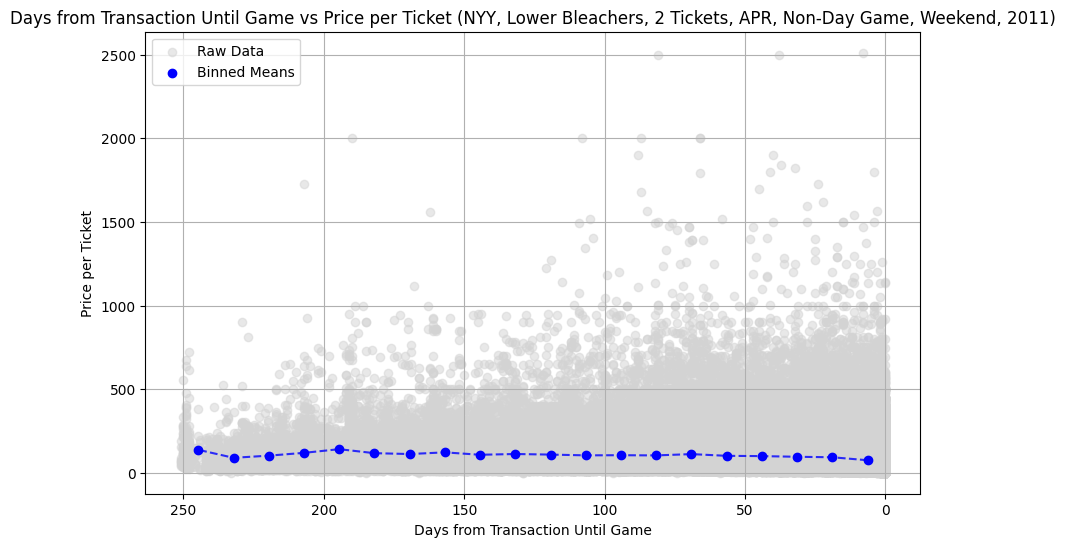
\includegraphics{images/10.png}

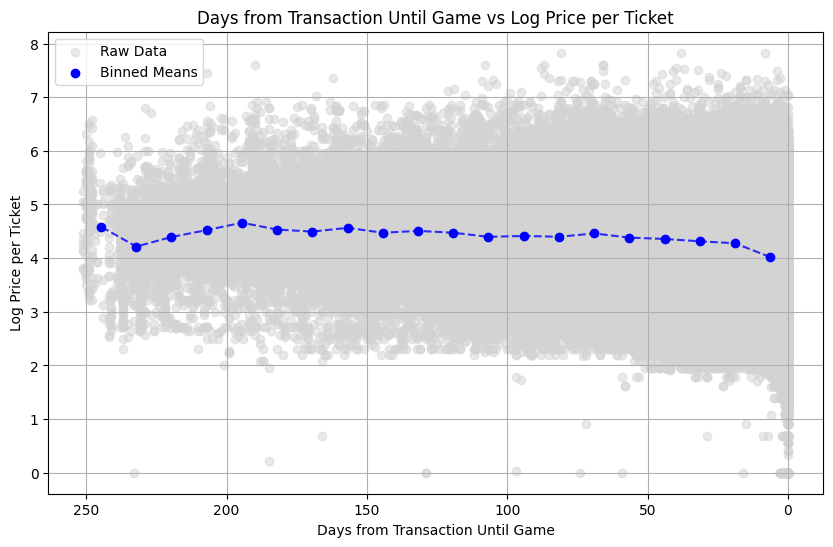
\includegraphics{images/8-01.png}

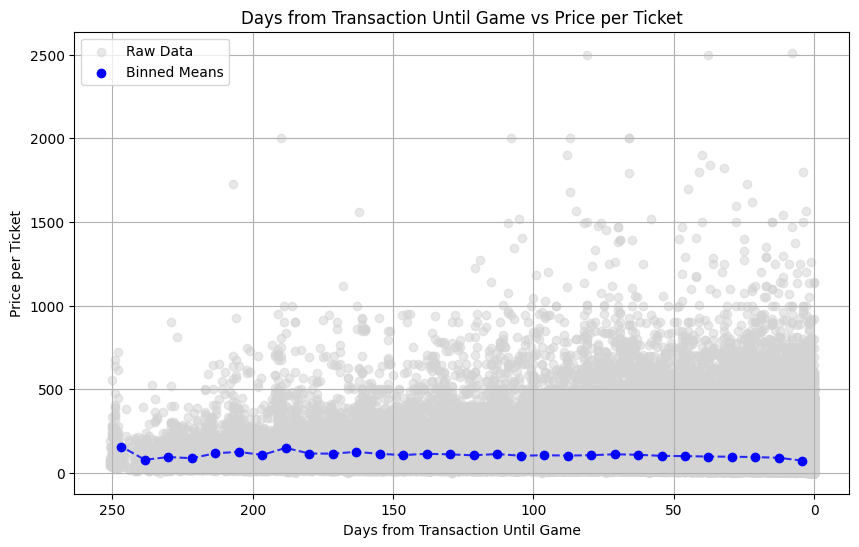
\includegraphics{images/7.png}

From this we see our regression results makes sense now. There are huge
outliers of people who pay more when game day is near (relative to when
game day is far). But on average people pay less when buying tickets
near game day. So to answer this question How do the prices consumers
pay for tickets change as the game date approaches (i.e., as the number
of days between transaction date and game date declines)? The initial
answer would be the prices \textbf{decrease} as game date approaches. To
further investigate the dynamic pattern, we would run a quasi ``event
study'' model to investigate. We show the distribution of transaction
and see there is bunching happening approximately every 8 days. There
are many reasons why this can be happening ranging from
discounts/promotions, timing of the games, etc. While we don't know why
exactly this is happening we can exploit these observations for our
event study model.

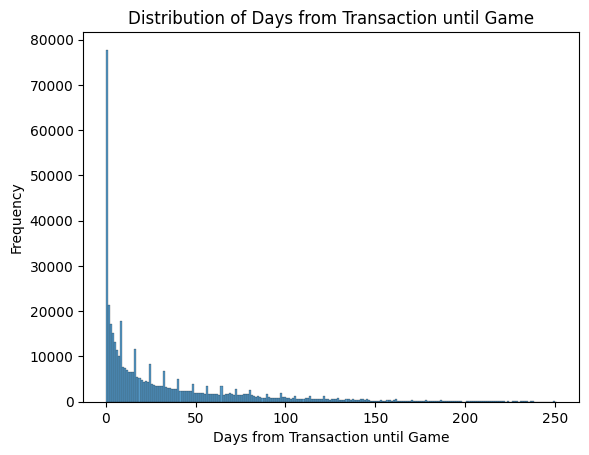
\includegraphics{images/6.png}

Using this observation we create our model.

\[
\text{price\_per\_ticket} = \beta_0 + \sum_{j=1}^{n} \beta_{1j} \cdot D_j \cdot \text{days\_until\_game} + \beta_2 \cdot \text{controls} + \beta_3 \cdot \text{num\_tickets} + \epsilon
\]

\subsection{Where:}\label{where}

\[
\mathbf{\mathrm{controls}} = \text{day\_game, weekend\_game, sectiontype, gamemonth, team, year}
\]

\begin{itemize}
\tightlist
\item
  \(\beta_0\) is the intercept.
\item
  \(\beta_{1j}\) is the coefficient for each range \(j\) of days from
  transaction until game:

  \begin{itemize}
  \tightlist
  \item
    \(D_1 = 1\) if days are in the range \(0-8\)
  \item
    \(D_2 = 1\) if days are in the range \(9-16\)
  \item
    \(D_3 = 1\) if days are in the range \(17-24\)
  \item
    \ldots{}
  \item
    \(D_n = 1\) for the last specified range (e.g., \(241-250\)).
  \end{itemize}
\item
  \(\beta_2 \cdot \mathbf{\text{controls}}\) represents a vector of
  control variables included in the model.
\item
  \(\beta_3\) is the coefficient for the number of tickets.
\item
  \(\epsilon\) is the error term.
\end{itemize}

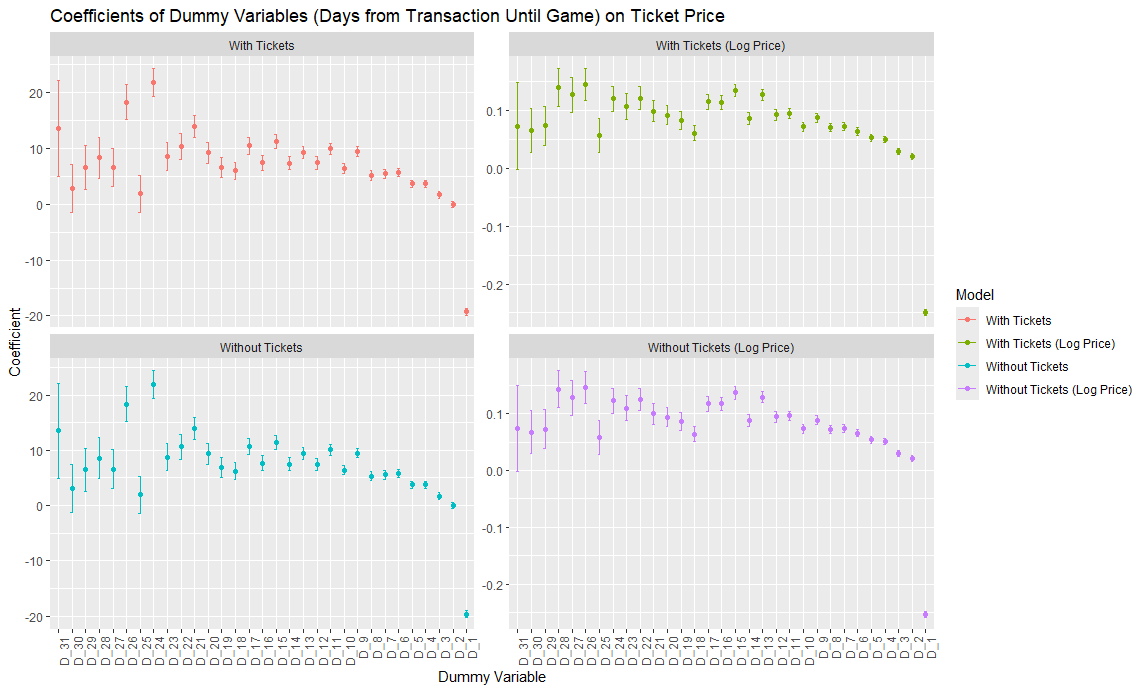
\includegraphics{images/12.png}

We see from this that the relationship may not be entirely linear. We
also see that ticket prices are in fact lower come one week before a
game, which supports previous results. One thing we did not take into
account for is the bias of human time perception. People typically think
of time between weeks, days and months, wherein overly long periods of
times are not referred to in weeks but in months. To study this, we run
the same model but take into account human biases, instead of cutting
the dummy variables in a 8 day basis, we cut up our dummy variables
based on human perceptions of months and weeks.

\[
\mathrm{price\_per\_ticket} = \beta_0 + \sum_{j=1}^{n} \beta_{1j} \cdot D_j \cdot \mathrm{days\_until\_game} + \beta_2 \cdot \mathrm{controls} + \beta_3 \cdot \mathrm{num\_tickets} + \epsilon
\]

\subsection{Where:}\label{where-1}

\[
\mathbf{\mathrm{controls}} = \mathrm{day\_game, weekend\_game, sectiontype, gamemonth, team, year}
\]

\begin{itemize}
\tightlist
\item
  \(\beta_0\) is the intercept.
\item
  \(\beta_{1j}\) is the coefficient for each range \(j\) of weeks and
  months from the transaction until the game:

  \begin{itemize}
  \tightlist
  \item
    \(D_1 = 1\) if the time until the game is in the range of 0-1 week
  \item
    \(D_2 = 1\) if the time until the game is in the range of 1-2 weeks
  \item
    \(D_3 = 1\) if the time until the game is in the range of 2-3 weeks
  \item
    \(D_4 = 1\) if the time until the game is in the range of 3-4 weeks
  \item
    \(D_5 = 1\) if the time until the game is in the range of 4-5 weeks
  \item
    \(D_6 = 1\) if the time until the game is in the range of 1-2 months
  \item
    \(D_7 = 1\) if the time until the game is in the range of 2-3 months
  \item
    \(D_8 = 1\) if the time until the game is in the range of 3-4 months
  \item
    \ldots{}
  \item
    \(D_n = 1\) if the time until the game is in the range of 8 to 8.3
    months, as the data concludes at 250 days.
  \end{itemize}
\item
  \(\beta_2 \cdot \mathbf{\text{controls}}\) represents a vector of
  control variables included in the model.
\item
  \(\beta_3\) is the coefficient for the number of tickets.
\item
  \(\epsilon\) is the error term.
\end{itemize}

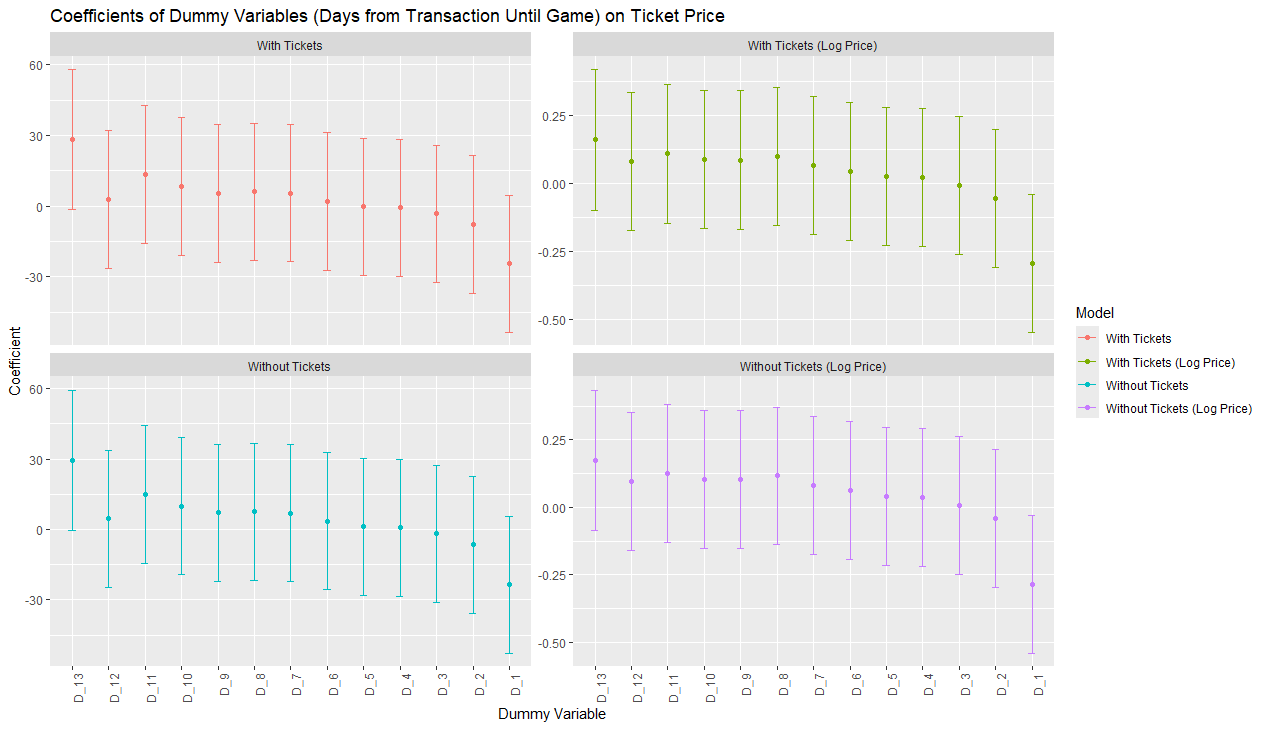
\includegraphics{images/13.png}

We see smoother and more observable relationship here. All this to
suggest that in fact, on average, the later you buy your tickets the
cheaper ticket prices would be. Next we study the year differences. We
look at the year coefficients of our main model.

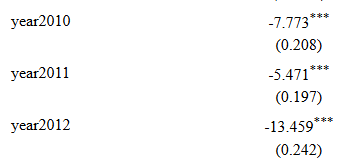
\includegraphics{images/14.png}

We see that there are significant year fixed effects that could be worth
investigating. Next, we run the same analysis restricting our
observations within each year.

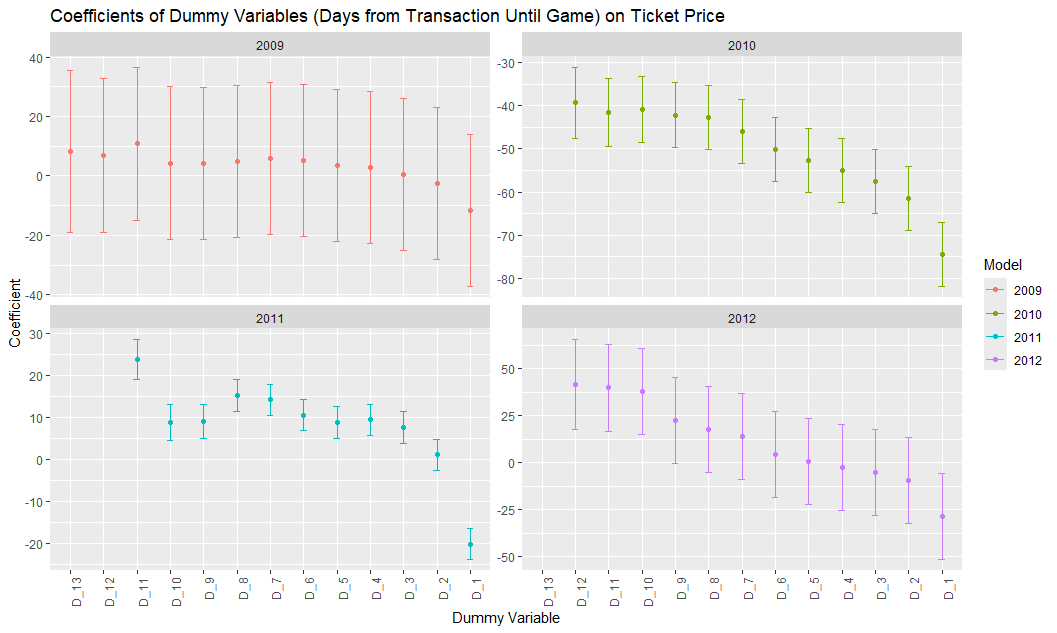
\includegraphics{images/15.png}

The observed trends reveal an interesting pattern: purchasing tickets
well in advance tends to result in higher ticket prices. However, there
are variations in this relationship over the years. For instance, in
2009, the standard error is notably large, indicating substantial
variability. During this year, some consumers were able to purchase
tickets far in advance (approximately 250 days before the game) at
prices comparable to those closer to game day.

In contrast, the dynamics shift in subsequent years, particularly in
2010, 2011, and 2012. The standard error becomes significantly smaller,
demonstrating greater consistency in pricing trends. As a result, a
clearer pattern emerges: tickets purchased closer to game day are
generally cheaper. By 2012, buying tickets just one week before the game
consistently results in lower prices, emphasizing the evolving dynamic
relationship between purchase timing and ticket cost.

\section{Task 2: Data Manipulation}\label{task-2-data-manipulation}

The data task took approximately 40 min.


  \bibliography{bibliography.bib}


\end{document}
